% !TEX root = HwXTemplate.tex


The diagram shown in Figure~\ref{Subset-sum-TM} is a non-deterministic Turing machine
that solves the subset sum problem in non-deterministic polynomial time. I will use this machine
as a motivating example when presenting the proof of the Cook-Levin Theorem showing
that the 3-CNF satisfaction problem is NP-complete. Accordingly, I thought it might be
useful for you to explore this Turing machine a bit before we discuss the proof.
	\begin{figure}
	\begin{center}
	%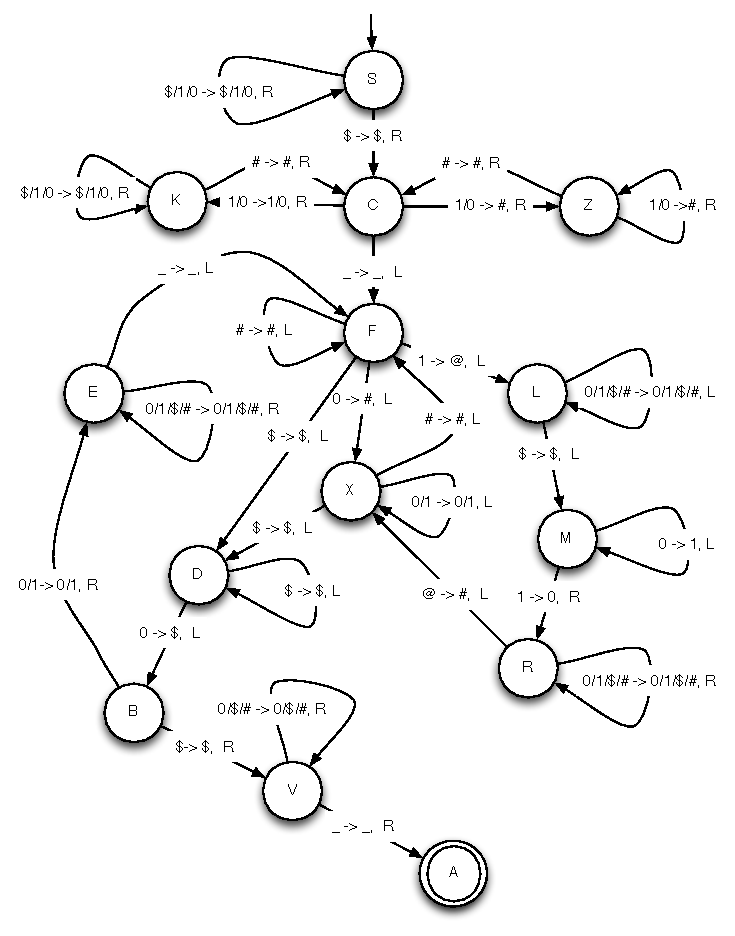
\includegraphics{../HwX/figs/SubsetSumPolyNTM.pdf}
	\end{center}
	%\caption{A NTM that decides Subset-sum}
	\label{Subset-sum-TM}
	\end{figure}
	
	The input this machine expects is a value N encoded in binary and surrounded by a pair of dollar signs (\$)
	followed by a list of integer values also encoded in binary but separated from one another and terminated
	by number signs (\#). Thus, the input $\$1001\$101\#100\#11\#10\#$ would represent the subset-sum
	question ``Is there a sublist of the numbers (5, 4, 3, 2) that adds up to 9?''

	In this figure, a notation of the form $0/1/\# \rightarrow 0/1/\#, L$ on a transition is meant as a shorthand
	meaning that the transition can be taken on any of the inputs 0, 1 or \# and that the symbols written
	if the transition is taken are 0, 1, and \# respectively. That is, this particular example says that on
	any of the symbols listed, the machine can move one square to the left while leaving the previous
	tape cell unchanged.
	
	This machine is fairly simple, but it does not employ the most obvious algorithm to solve
	the problem. Unfortunately, like all too many programmers before me, I failed to include
	good comments explaining the algorithm the Turing machine shown in the figure uses.
	
	The ``obvious'' algorithm is to first randomly cross out some list of the 
	numbers provided by replacing their digits with
	number signs (my non-obvious algorithm starts by performing exactly this process). 
	Then, the obvious way to verify that the random guesses made generated a correct solution
	would be to repeatedly subtract one from the number between the dollar signs 
	and from one of the numbers that were not crossed out initially to verify that this process
	leads to a situation in which all of the non-crossed out numbers get reduced to zeros
	at the same point that the number between the dollar signs reaches zero.
	\begin{enumerate}
	\item Help me out! Generate the missing documentation. That is, please give a brief, informal
		description of the algorithm implemented by the Turing machine in Fig.~\ref{Subset-sum-TM}
		and justify its correctness.
	\item Analyze the running time of my Turing machine and give a bound on its worst-case running time
		as a function of the size of its input string.
	\item Explain why I used this Turing machine as my lecture example rather than the ``obvious'' one.
		It turns out that although the obvious one might have been easier to implement, it would
		not have been an appropriate example.
	\end{enumerate}


\begin{solution}

% Place your answers here
\begin{enumerate}
	\item The top four states takes care of guessing the subset of numbers that are part of the sum that add up to the target. It does this by skipping the target number and guessing which numbers to keep denoted by the $K$ and which to get rid of denoted by the $Z$. It keeps numbers by just moving to the pound sign to the right of the number, and it removes a number by replacing every binary digit with a $\#$.\\
	This machine scans for odd numbers in the guessed sublists and makes them even by subtracting one. It also subtracts one from the target to make sure that the sum of the sublist still equals the target. Once all numbers are even, it divides them all by 2.\\
	Once the machine reaches the end of the input it integer divides all numbers by 2. An odd number is divided by 2 by placing an $@$ on the right-most bit, then subtracting one from the target, and replacing the $@$ with a $\#$. Even numbers are divided by replacing the right-most zero with a $\#$. It does this until all the numbers in the sublist are even. Once this happens, it checks that the target is even and divides it by 2. If the target still has more digits to process, the machine begins the next right to left scan. On the other hand, it scans to the right to make sure that all other digits have also been deleted. If so, the input is accepted.
	\item Run Time: $O(n^2)$.\\
	The steps taken by states $L,M,\mbox{ and }R$ take $O(2n)$ steps. Subtracting 1 from both the target and a value in the sublist requires a scan from the first 1 to the right of the tape to the left-most digit from the target. This is at most $|X|$ steps. The machine must then travel all the way back to the $@$ which is another $|X|$ steps away at most. This is done for all odd numbers which is at most $|X|$ to find, hence the $O(n^2)$ runtime.\\
	The same runtime applies to dividing the target value by 2, as it has to move to the right of the tape which takes $O(n)$ time. This occurs $O(n)$ times for a total of $O(n^2)$.
\end{enumerate}


\end{solution}
